\section{Results}
\label{sec:result}

I run a Metropolis-Hastings algorithm for 2,000,000 iterations, choosing the proposal step size so that the acceptance rate falls within 20\% and 50\% \citep{Hoff2009}. To reduce autocorrelation between iterations, I thin the sample and only keep the sampled values every 100 steps, resulting in a final posterior sample of 20,000.

\subsection{Results on Firms' Preferences}

\Cref{fig:traceplot_alpha} show the trace plots of $\alpha$, firms' preference parameters for countries' log GDP, log GDP per capita, democracy, and labor quality. The plots show that the MCMC chains converge after the 10000\textsuperscript{th} iterations, except for the average years of schooling. Thus, our interpretation for this variable has to be more cautious.

\begin{figure}[!ht]
\centering
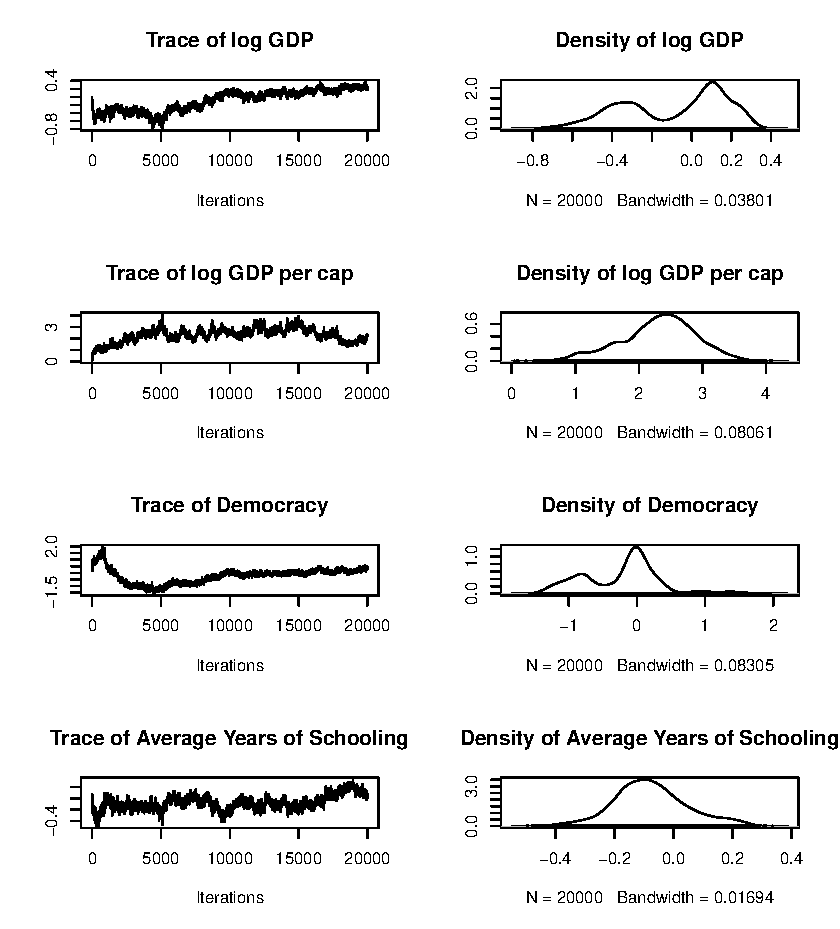
\includegraphics[width=\textwidth,keepaspectratio]{../figure/traceplot_alpha}
\caption{Traceplot of firms' preferences for countries' characteristics.}
\label{fig:traceplot_alpha}
\end{figure}

\Cref{tab:posterior_alpha} report the posterior means and quantiles of firms' preference parameters. The posterior means can be interpreted naturally in the utility space as the relative weights that firms assign to countries' characteristics.\footnote{In the utility space, the scale of the parameters do not matter. Consider two scenarios: 1) country A offers 10 ``utilities'' while country B offers 50; 2) country A offers 1 ``utility'' while country B offers 5. These two scenarios are identical since the firm will choose country B over country A. For this reason, we focus on interpreting preference parameters as relative weights.} For example, since the value of firms' preference for democracy is 0.02 and for log GDP per capita is 2.5, it means that being a democracy is worth 0.02 / 2.5 = 0.008 of 1 unit increase in log GDP. Interpreting on the level scale, it means that being a democracy is worth 0.305 / 0.025 = 12.2 times a 1\% increase in GDP.

However, looking at the posterior quantiles, we find that only GDP per capita is a statistically significant factor in MNCs' utilities. While this finding contradicts existing theories on the determinants of FDI, it comports with the latest empirical evidence. After correcting for selection bias and using Bayesian model averaging to select robust determinants of FDI, \citet{Eicher2012} also finds that host country's size, regime type, and educational attainment do not play an important role in attracting FDI.

\begin{table}[!ht]
\centering
\begin{tabular}{l|lllll}
                           & 2.5\% & 25\%  & 50\%  & 75\% & 97.5\% \\ \hline
log GDP                    & -0.05 & 0.07  & 0.12  & 0.19 & 0.29   \\
log GDP per cap            & 1.53  & 2.15  & 2.50  & 2.84 & 3.44   \\
Average Years of Schooling & -0.23 & -0.13 & -0.06 & 0.06 & 0.23   \\
Democracy                  & -0.24 & -0.08 & 0.02  & 0.14 & 0.40  
\end{tabular}

\caption{The posterior quantiles of firms' preferences for countries' characteristics.}
\label{tab:posterior_alpha}
\end{table}

\subsection{Results on Countries' Preferences}

Due to the small number of Japanese firms locating in certain countries, the MCMC chains for their parameters converge much slowly, if at all. For example, Myanmar has only seven Japanese firms. Its traceplots show that the MCMC chains do not seem to converge even after 20,000 iterations (\Cref{fig:traceplot_myanmar}). Given the lack of convergence, the results in this section remain speculative.

\begin{figure}[!ht]
\centering
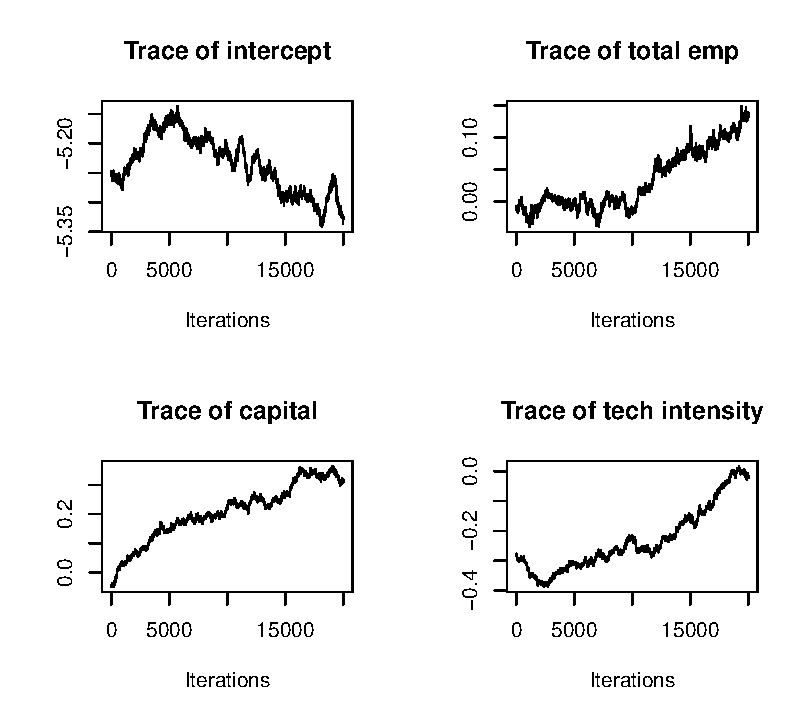
\includegraphics[width=\textwidth,keepaspectratio]{../figure/traceplot_myanmar}
\caption{Traceplot of Myanmar's preferences for MNCs' characteristics.}
\label{fig:traceplot_myanmar}
\end{figure}

To test the hypothesis that only governments with a long time horizon actively seeks high tech MNCs, I proxy time horizon with the age of the executive's party. A long-running party has an extended time horizon for two reasons. First, given its longevity, it is possible for the party to come back to power in the future, reaping the benefits of its investment in attracting high-tech FDI. Second, given that a long-running party has a persistent, identifiable brand, it can more easily claim the credit for attracting high-tech MNCs even if the benefit only materializes many years later.

\Cref{fig:preference_for_tech} attempts to show the positive relationship between a government's time horizon and its preference for high-tech MNCs. While there is a positive slope, the sample size of countries is too small to make any definitive claim.

\begin{figure}[!ht]
\centering
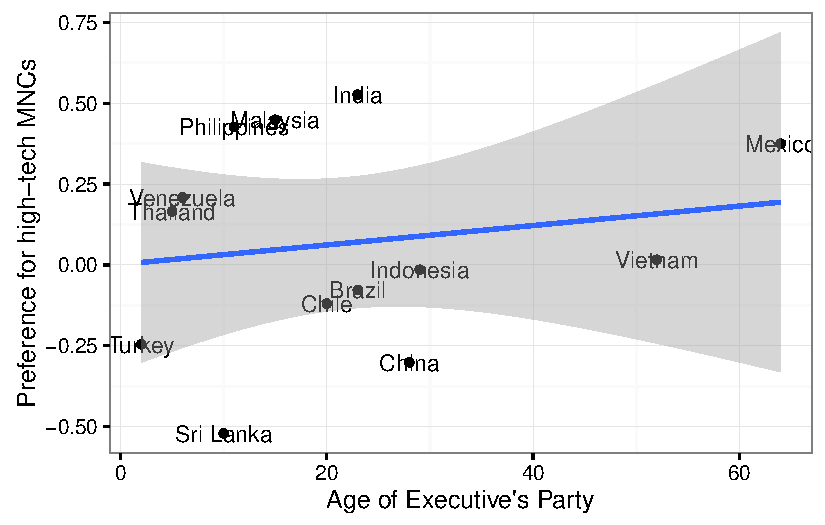
\includegraphics[width=0.7\textwidth,keepaspectratio]{../figure/preference_for_tech}
\caption{The relationship between a government' time horizon and its preference for high-tech MNCs.}
\label{fig:preference_for_tech}
\end{figure}
